\chapter{Mock-up}
\label{s:mockup}


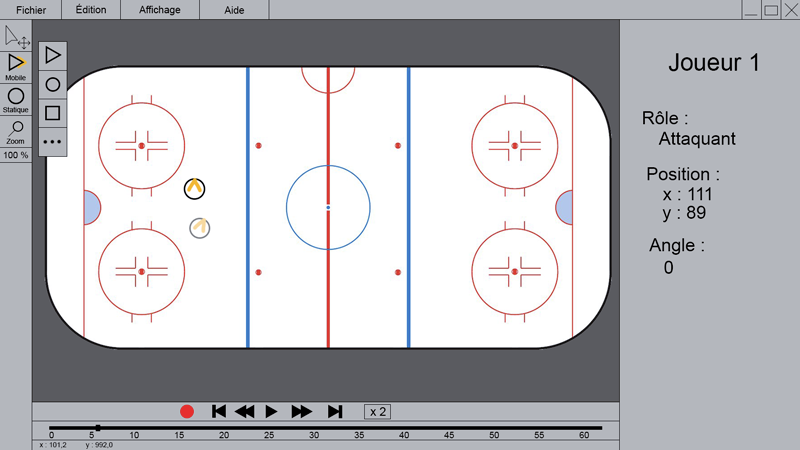
\includegraphics[scale=0.55]{mockup/mockup.png}

\section{Description}

\subsection{Section du centre}

Cette section est celle où la scène est affiché. Dans le fond de la scène, s'affiche le terrain. C'est dans cette section où les éléments sont placés. En plaçant la sourie sur un élément, un icône s'affiche. En appuyant dessus, il est possible de modifier l'angle de l'élément.

\subsection{Section de droite}

Cette section contient les paramètres de l'élément actuellement sélectionné. Le "Joueur 1" est le nom de l'élément. C'est un champ texte modifiable. Le "Attaquant" est le rôle du joueur. C'est un comboBox dans lequel les valeurs sont celles entrée dans les paramètres du sport. La position en x et en y de l'élément est modifiable via des champs numériques modifiables. L'angle aussi modifiable en utilisant un champ numérique dont la valeur est restreinte entre -360 et 360. Les valeurs négatives sont converties en valeurs positives.

\subsection{Section du bas}

Cette section permet de gérer la visualisation de la stratégie. Le cercle rouge permet de démarrer l'enregistrement de la stratégie. Les autres boutons sont les boutons traditionnels lors du visionnement de vidéo. Le x2 permet de modifier la vitesse de défilement lors d'avance rapide et de recule. 

En dessous se trouve une ligne du temps. Le rectangle noir, le curseur, indique quel image est affiché dans la scène. En le modifiant, l'image affiché dans la scène change. 

\subsection{Section de gauche}

Cette section contient les boutons permettant d'ajouter des éléments à la scène. C'est la barre d'outil. Le premier à partir du haut est celui utilisé pour déplacer les éléments. Le second sert à créer les éléments mobiles. Le troisième sert à créer les éléments statiques. En maintenant un clic sur le second et le troisième bouton, des icônes apparaissent à droite. Ils permettent de modifier l'élément qui sera ajouter à la scène grâce aux outils d'ajout d'éléments. Le quatrième bouton sert à zoomer sur la scène. Juste en dessous se trouve un champ numérique, permettant de modifier le zoom. 